\documentclass[conference]{IEEEtran}

\let\labelindent\relax
\usepackage{amsmath}
\usepackage{amsfonts}
%\usepackage[colorlinks=true, citecolor=blue, urlcolor=cyan, linkcolor=red]{hyperref}
\usepackage{amssymb}
\usepackage{amsmath,amssymb,amscd,epsfig,amsfonts,rotating}
\usepackage{graphicx}
\usepackage{epstopdf}
\usepackage{subfigure}
\usepackage{multirow}
\usepackage{booktabs}
\usepackage{color,xcolor}
\usepackage{url}
\usepackage{amsmath,amscd,amsbsy,amssymb,latexsym,url,bm}
\usepackage{epsfig,epstopdf,graphicx,subfigure}
\usepackage{enumitem,balance,mathtools}
\usepackage{wrapfig}
\usepackage{mathrsfs, euscript}
\usepackage{algorithm}
\usepackage{algorithmic}
\usepackage{amssymb}
\usepackage{ifpdf}
\usepackage{diagbox}
\usepackage{caption}
\usepackage{makecell}
\usepackage{extarrows}

\hyphenation{op-tical net-works semi-conduc-tor}

\newcommand{\bs}{\boldsymbol}
\newcommand{\bW}{\bs{W}}
\newcommand{\bb}{\bs{b}}
\newcommand{\bl}{\bs{l}}
\newcommand{\bz}{\bs{z}}
\newcommand{\bp}{\bs{p}}
\newcommand{\bx}{\bs{x}}
\newcommand{\Bf}{\bs{f}}
\newcommand{\btheta}{\bs{\theta}}
\newcommand{\mR}{\mathbb{R}}
\newcommand{\sigmoid}{\text{sigmoid}}
%\newcommand{\tanh}{\text{tanh}}
\newcommand{\relu}{\text{relu}}

\newcommand{\yanru}[1]{{\bf \color{blue} [[Yanru says ``#1'']]}}
\newcommand{\han}[1]{{\bf \color{yellow} [[Han says ``#1'']]}}
\newcommand{\weinan}[1]{{\bf \color{red} [[Weinan says ``#1'']]}}
\newcommand{\kan}[1]{{\bf \color{green} [[Kan says ``#1'']]}}
\newcommand{\rocky}[1]{{\bf \color{pink} [[Rocky says ``#1'']]}}

%\linespread{1.01}

\begin{document}

\title{Product-based Neural Networks for User Response Prediction}


% author names and affiliations
% use a multiple column layout for up to three different
% affiliations
\author{
\IEEEauthorblockN{Yanru Qu, Han Cai, Kan Ren, Weinan Zhang, Yong Yu}
\IEEEauthorblockA{Shanghai Jiao Tong University\\
	\{kevinqu, hcai, kren, wnzhang, yyu\}@apex.sjtu.edu.cn}
\and
\IEEEauthorblockN{Ying Wen, Jun Wang}
\IEEEauthorblockA{University College London\\
\{ying.wen, j.wang\}@cs.ucl.ac.uk}
}


% make the title area
\maketitle

% As a general rule, do not put math, special symbols or citations
% in the abstract
\begin{abstract}
Predicting user responses, such as clicks and conversions, is of great importance and has found its usage in many Web applications including recommender systems, web search and online advertising. The data in those applications is mostly categorical and contains multiple fields; a typical representation is to transform it into a high-dimensional sparse binary feature representation via one-hot encoding.
Facing with the extreme sparsity, traditional models may limit their capacity of mining shallow patterns from the data, i.e. low-order feature combinations. Deep models like deep neural networks, on the other hand, cannot be directly applied for the high-dimensional input because of the huge feature space.
In this paper, we propose a Product-based Neural Networks (PNN) with an embedding layer to learn a distributed representation of the categorical data, a product layer to capture interactive patterns between inter-field categories, and further fully connected layers to explore high-order feature interactions.
Our experimental results on two large-scale real-world ad click datasets demonstrate that PNNs consistently outperform the state-of-the-art models on various metrics.
\end{abstract}

%We present two types of PNNs in terms of the inner and outer product of embedded vectors, and prove that these models can be efficiently implemented under linear time and space complexity.

%\begin{abstract}
%User response prediction is now playing a crucial role in many information retrieval tasks, including recommender systems, web search and online advertising.
%The data to deal with is mostly in a multi-field categorical form, which is normally transformed into a high-dimensional sparse binary feature representation via one-hot encoding.
%Working on such sparse binary feature inputs, traditional models are limited in mining high-order latent patterns.
%In this paper, we propose a novel architecture of deep neural networks, namely Product-based Neural Network (PNN), which can automatically learn high-order latent patterns and pairwise feature interactions.
%The product operations we introduced broaden networks' ability in dealing with multi-field categorical data.
%Our experimental results on two large-scale real-world datasets demonstrate that PNNs consistently outperform state-of-the-art models on various metrics.
%\end{abstract}

%Moreover, the features that these models utilize are always discrete categorical data, which requires high learning ability of the models.
% no keywords

\IEEEpeerreviewmaketitle


\section{Introduction}\label{sec:intro}
% user response prediction plays a key role in many systems
Learning and predicting user response now plays a crucial role in many personalization tasks in information retrieval (IR), such as recommender systems, web search and online advertising. The goal of user response prediction is to estimate the probability that the user will provide a predefined positive response, e.g. clicks, purchases etc., in a given context
\cite{menon2011response}.
This predicted probability indicates the user's interest on the specific item such as a news article, a commercial item or an advertising post, which influences the subsequent decision making such as document ranking \cite{xue2004optimizing} and ad bidding \cite{zhang2014optimal}.

%Taking online advertising as an example, click-through rate (CTR) estimation will be utilized to calculate a bid price in an ad auction \cite{zhang2014optimal, perlich2012bid}.
%Naturally, it is much desirable to gain accurate prediction to not only improve the user experience, but also boost the volume and profit for the service providers.

% traditional models: linear and non linear
% shallow feature pattern
% interactive patterns mining
The data collection in these IR tasks is mostly in a multi-field categorical form, for example, \texttt{[Weekday=Tuesday, Gender=Male, City=London]}, which is normally transformed into high-dimensional sparse binary features via one-hot encoding \cite{he2014practical}.
For example, the three field vectors with one-hot encoding are concatenated as
\[ \underbrace{[0,1,0,0,0,0,0]}_{\texttt{Weekday=Tuesday}}\underbrace{[0,1]}_{\texttt{Gender=Male}} \underbrace{[0,0,1,0,\ldots,0,0]}_{\texttt{City=London}}.\]
Many machine learning models, including linear logistic regression \cite{lee2012estimating}, non-linear gradient boosting decision trees \cite{he2014practical} and factorization machines \cite{ta2015factorization}, have been proposed to work on such high-dimensional sparse binary features and produce high quality user response predictions.
%User response prediction can be regarded as a binary classification task in practice, i.e. positive response or not \cite{richardson2007predicting,graepel2010web}.
%LR, GBDT and FM, have been proved success in industrial applications.
%The linear models are easy to implement and with high efficiency.
However, these models highly depend on feature engineering in order to capture high-order latent patterns \cite{cui2011bid}.
%To tackle this problem, non-linear models such as are studied to explore feature interactions. These algorithms deal with a huge number of sparse features with one-hot encoding but they still suffer from modeling limit so as not to fully explore non-trivial patterns in the multi-field categorical data.

% deep learning for data representation
Recently, deep neural networks (DNNs) \cite{lecun2015deep} have shown great capability in classification and regression tasks, including computer vision \cite{krizhevsky2012imagenet}, speech recognition \cite{graves2013speech} and natural language processing \cite{mikolov2013distributed}. It is promising to adopt DNNs in user response prediction since DNNs could automatically learn more expressive feature representations and deliver better prediction performance.
In order to improve the multi-field categorical data interaction, \cite{zhang2016deep} presented an embedding methodology based on pre-training of a factorization machine. Based on the concatenated embedding vectors, multi-layer perceptrons (MLPs) were built to explore feature interactions. However, the quality of embedding initialization is largely limited by the factorization machine.
More importantly, the ``add'' operations of the perceptron layer might not be useful to explore the interactions of categorical data in multiple fields. Previous work \cite{menon2011response,ta2015factorization} has shown that local dependencies between features from different fields can be effectively explored by feature vector ``product'' operations instead of ``add'' operations.


%In capturing the multi-field categorical data interactions, the authors in \cite{zhang2016deep} proposed a DNN solution for CTR estimation, which integrates FM as an embedding initialization in neural networks.
%The authors in \cite{liu2015convolutional} proposed a convolutional model to predict ad click, being able to model single and sequential behaviors. Besides, RNN is applied in learning sequential data \cite{zhang2014sequential}. These works have shown the potential of DNNs in user response prediction.

%\rocky{The specific models of DNN could be put in the Related Work part}

To utilize the learning ability of neural networks and mine the latent patterns of data in a more effective way than \text{MLPs,} in this paper we propose Product-based Neural Network (PNN) which (i) starts from an embedding layer without pre-training as used in \cite{zhang2016deep}, and (ii) builds a product layer based on the embedded feature vectors to model the inter-field feature interactions, and (iii) further distills the high-order feature patterns with fully connected MLPs.
We present two types of PNNs, with inner and outer product operations in the product layer, to efficiently model the interactive patterns.

We take CTR estimation in online advertising as the working example to explore the learning ability of our PNN model. The extensive experimental results on two large-scale real-world datasets demonstrate the consistent superiority of our model over state-of-the-art user response prediction models \cite{ta2015factorization,liu2015convolutional,zhang2016deep} on various metrics.

%To utilize the learning ability of DNNs and mine the latent patterns of data in a more effective way than \text{MLPs,}, in this paper we propose Product-based Neural Network (PNN) which explores the inter-field feature interactions via vector production, a.k.a., the product layers. We introduce the product layers in neural networks for several reasons: a). traditional neural networks, local information is burried in the global summition, b). taking binary inputs as electronical signals, it is natural to apply addition as ``OR" gate, and multiplication as ``AND" gate, c). different from learning feature expressions, we propose PNN to learn rule expressions.

%We present two types of PNNs, with inner and outer product operations in the product layer, to efficiently model the interactive patterns.
%We take CTR estimation in online advertising as the working example to evaluate our PNN models. The extensive experimental results on two large-scale real-world datasets demonstrate the consistent superiority of our model over state-of-the-art models \cite{ta2015factorization,liu2015convolutional,zhang2016deep} on various metrics.
%\rocky{Here could introduce more about PNN, what is special in the PNN and what function/advantage it has}

% contribution

%To sum up, our contributions can be highlighted as below:
%\begin{itemize}
%\item We present an effective DNN model for user response prediction, which significantly improves the prediction performance.
%\item PNN can efficiently learn distributed data representations on multi-field categorical data.
%\item We demonstrates approximation solutions for pairwise operations in PNN, making it efficient and scalable.
%\end{itemize}

% paper schedule
%The rest of this paper is organized as follows. In Section~\ref{sec:related} we discuss some related work on user response learning and prediction. In Section~\ref{sec:methodology} we present our PNN models in detail. The experimental setup and results are illustrated in Section~\ref{sec:experiment}. We finally conclude this paper and make some discussions about the future work in Section~\ref{sec:conclusion}.


\section{Related Work}\label{sec:related}
%CTR estimation is a typical user response prediction problem.
%For example, the CTR estimation is usually utilized to derive the budget allocation of the advertisers \cite{richardson2007predicting}.
The response prediction problem is normally formulated as a binary classification problem with prediction likelihood or cross entropy as the training objective \cite{richardson2007predicting}.
Area under ROC Curve (AUC) and Relative Information Gain (RIG) are common evaluation metrics for response prediction accuracy \cite{graepel2010web}.
%Typically, the response prediction problem is formulated as a binary classification problem with prediction likelihood/cross entropy as the training objective \cite{richardson2007predicting,graepel2010web,agarwal2010estimating,oentaryo2014predicting}.
From the modeling perspective, linear logistic regression (LR) \cite{lee2012estimating,ren2016user} and non-linear gradient boosting decision trees (GBDT) \cite{he2014practical} and factorization machines (FM) \cite{ta2015factorization} are widely used in industrial applications. However, these models are limited in mining high-order latent patterns or learning quality feature representations.
%There are also some learning algorithms dealing with sparse binary inputs, including Bayesian probit regression \cite{graepel2010web}, FTRL \cite{ta2015factorization}.
%These models perform well on traditional prediction tasks, however, the data are facing the problem of sparsity and large bias \cite{he2014practical}.
%It is natural to seek for a model with better learning ability and expression power.
%\weinan{This section is too short. Write more detailed work here.}

Deep learning is able to explore high-order latent patterns as well as generalizing expressive data representations \cite{mikolov2013distributed}.
The input data of DNNs are usually dense real vectors, while the solution of multi-field categorical data has not been well studied. Factorization-machine supported neural networks (FNN) was proposed in \cite{zhang2016deep} to learn embedding vectors of categorical data via pre-trained FM.
Convolutional Click Prediction Model (CCPM) was proposed in \cite{liu2015convolutional} to predict ad click by convolutional neural networks (CNN). However, in CCPM the convolutions are only performed on the neighbor fields in a certain alignment, which fails to model the full interactions among non-neighbor features.
Recurrent neural networks (RNN) was leveraged to model the user queries as a series of user context to predict the ad click behavior \cite{zhang2014sequential}.
%However, sequential data is not always available.
%, it has not shown the generalization for common user response prediction.
Product unit neural network (PUNN) \cite{engelbrecht1999training} was proposed to build high-order combinations of the inputs. However, neither can PUNN learn local dependencies, nor produce bounded outputs to fit the response rate.
%Moreover, these  model do not consider much about the interactive patterns within data.
%\weinan{add references on product layers in neural networks.}

In this paper, we demonstrate the way our PNN models learn local dependencies and high-order feature interactions.
%, and we provide approximation solutions in reducing the polynomial feature space

\section{Deep Learning for CTR Estimation}\label{sec:methodology}

We take CTR estimation in online advertising \cite{richardson2007predicting} as a working example to formulate our model and explore the performance on various metrics. The task is to build a prediction model to estimate the probability of a user clicking a specific ad in a given context.
%\rocky{put this sentence in related work part}
%As illustrated in Figure~,

Each data sample consists of multiple fields of categorical data such as user information (\texttt{City}, \texttt{Hour}, etc.), publisher information (\texttt{Domain}, \texttt{Ad slot}, etc.) and ad information (\texttt{Ad creative ID}, \texttt{Campaign ID}, etc.) \cite{zhang2014real}. All the information is represented as a multi-field categorical feature vector, where each field (e.g. \texttt{City}) is one-hot encoded as discussed in Section~\ref{sec:intro}.
Such a field-wise one-hot encoding representation results in curse of dimensionality and enormous sparsity \cite{zhang2016deep}. Besides, there exist local dependencies and hierarchical structures among fields \cite{menon2011response}.

%The data for CTR estimation is always in a multi-field categorical form, which is normally transformed into high-dimensional sparse binary features via one-hot encoding.
%\rocky{refine this part introduction of data and put it in the Introduction}
%Thus, formally speaking, we can define CTR Estimation as a binary classification problem where the inputs are sparse binary features and the output is the predicted probability of click.
%And we want to solve this problem in a deep learning framework.
%In general the difficulties in mutli-field categorical data lie in
%To tackle the sparsity problem, an embedding layer is introduced to learn a low-dimensional real-valued representation for each field.
Thus we are seeking a DNN model to capture high-order latent patterns in multi-field categorical data. And we come up with the idea of product layers to explore feature interactions automatically. In FM, feature interaction is defined as the inner product of two feature vectors \cite{rendle2010factorization}.

The proposed deep learning model is named as Product-based Neural Network (PNN). In this section, we present PNN model in detail and discuss two variants of this model, namely Inner Product-based Neural Network (IPNN), which has an inner product layer, and Outer Product-based Neural Network (OPNN) which uses an outer product expression.

%Ad. features are usually numerical or categorical, e.g. size=480, city=London, among which categorical features are usually represented via one-hot encoding. Though simple and efficient, one-hot encoding results in enormous sparsity, e.g. a single data instance may have millions of input values while only tens of positive units.

%Besides, Ad. features are also hierarchical. Ad. features come from demand side and supply side. For the supply side, fetures are collected from users, publishers, and SSPs. For the demand side, features are collected from Ad. itself, advertisers, and DSPs.

\subsection{Product-based Neural Network}
%In this section, we present our Product Neural Networks (PNNs) in detail. And in general, PNN is a binary classifier with capacity of capturing sparse and hierarchical features.

%In dealing with sparse data, FM's outstanding performance proves the advantages of quadratic feature combination. FNN and CCPM prove neural networks' advantages in capturing abstract levels.

%We come up with the idea of product layers, which explores quadratic feature combinations automatically, expanding neural networks' learning capacity. PNN is thus named after the product layers.

\begin{figure}[t]
	\centering
	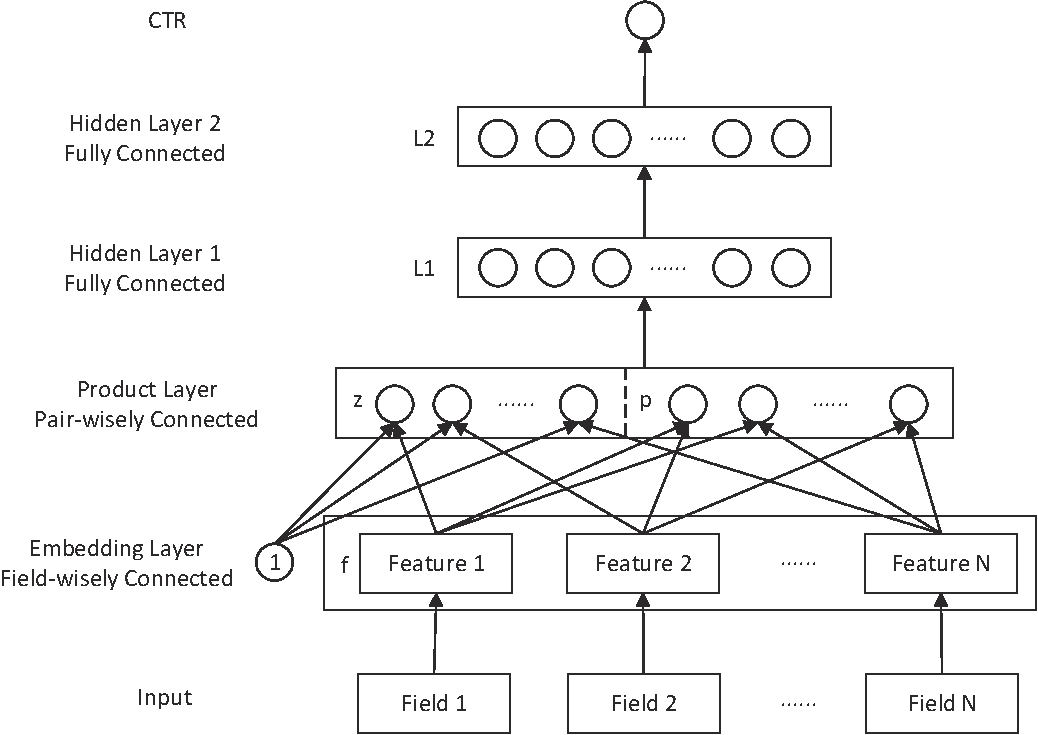
\includegraphics[width=1\columnwidth]{figure/pnn-arch-v-crop.pdf}
	\caption{Product-based Neural Network Architecture.}\label{fig:pnn}
\end{figure}

The architecture of the PNN model is illustrated in Figure~\ref{fig:pnn}.
%\kan{explanation of $D_i$}
%In general, by passing through the embedding layer, the input one-hot encoded fields are converted to low-dimensional real-valued feature vectors, which are pairwisely connected in the product layer.
%Then the real-valued feature vectors and their product results compose the input of latter fully connected layers.
%In the remaining part this section, we present the structure of product layers in detail.
%In terms of features vectors produced by the embedding layer, we propose two variants of PNN: the PNN-I based on vector inner product, and the PNN-II based on vector outer product. Before we investigate the details of product layers, we give a top-down view of the PNN network.
From a top-down perspective, the output of PNN is a real number $\hat{y} \in ( 0, 1 )$ as the predicted CTR:
\begin{equation}
\hat{y} = \sigma(\bW_3 \bl_2 + b_3), \label{eq:output}
\end{equation}
where $\bW_3 \in \mR^{1 \times D_2}$ and $b_3 \in \mR$ are the parameters of the output layer, $\bl_2 \in \mR^{D_2}$ is the output of the second hidden layer, and $\sigma(x)$ is the sigmoid activation function: $\sigma(x)= 1 / (1 + e^{-x})$. And we use $D_i$ to represent the dimension of the $i$-th hidden layer.

The output $\bl_2$ of the second hidden layer is constructed as
\begin{equation}
\bl_2 = \relu(\bW_2 \bl_1 + \bb_2),
\end{equation}
%where $\bW_2 \in \mR^{D_2 \times D_1}$ and $\bb_2 \in \mR^{D_2}$ are the parameters of the first hidden layer, and
where $\bl_1 \in \mR^{D_1}$ is the output of the first hidden layer. The rectified linear unit (relu), defined as $\relu(x) = \max(0, x)$, is chosen as the activation function for hidden layer output since it has outstanding performance and efficient computation.
%, which will be discussed in Section~\ref{sec:arch}.

The first hidden layer is fully connected with the product layer. The inputs to it consist of linear signals $\bl_z$ and quadratic signals $\bl_p$. With respect to $\bl_z$ and $\bl_p$ inputs, separately, the formulation of $\bl_1$ is:
\begin{align}\label{eq:l1-formula}
\bl_1 &= \relu(\bl_z + \bl_p + \bb_1),
\end{align}
%where $W_1$ is the parameter of the first hidden layer, $b_1$ is the bias, $z$ represents the feature vectors, $p$ represents the product terms, and $\begin{bmatrix} z \\ p \end{bmatrix}$ is the concatenation of both $z$ and $p$. Relu (Rectified Linear Unit) function, defined as $\relu(x) = max(0, x)$, is used here because we find this activation function outperforms others in both efficiency and performance.
where all $\bl_z$, $\bl_p$ and the bias vector $\bb_1 \in \mR^{D_1}$.

Then, let us define the operation of tensor inner product:
\begin{align}
\bs{A} & \odot \bs{B} \triangleq \sum_{i,j} \bs{A}_{i,j} \bs{B}_{i,j},
\end{align}
where firstly element-wise multiplication is applied to $\bs{A}, \bs{B}$, then the multiplication result is summed up to a scalar. After that,
$\bl_z$ and $\bl_p$ are calculated through $\bz$ and $\bp$, respectively:
\begin{align}\label{eq:l1-lz-lp}
\bl_z &= \begin{pmatrix}
l_z^1, l_z^2, \ldots, l_z^n, \ldots , l_z^{D_1}
\end{pmatrix}, \qquad l_z^n = \bW_z^n \odot \bz\\
\bl_p &= \begin{pmatrix}
l_p^1, l_p^2, \ldots, l_p^n, \ldots , l_p^{D_1}
\end{pmatrix}, \qquad l_p^n = \bW_p^n \odot \bp  \nonumber
\end{align}
%\weinan{very unclear! what is $\bs{A}_{i \ldots j}$? what is $\sum_{i \ldots j}$?}
where $\bW_z^n$ and $\bW_p^n$ are the weights in the product layer, and their shapes are determined by $\bz$ and $\bp$ respectively.

By introducing a ``1" constant signal, the product layer can not only generate the quadratic signals $\bp$, but also maintaining the linear signals $\bz$, as illustrated in Figure \ref{fig:pnn}. More specifically,
\begin{align}
\bz &= \begin{pmatrix}
\bz_1, \bz_2, \ldots, \bz_N
\end{pmatrix}
\triangleq \begin{pmatrix}
\Bf_1, \Bf_2, \ldots, \Bf_N
\end{pmatrix}, \\
\bp	&=
\{
\bp_{i, j}
\}, i = 1...N, j = 1...N,
\end{align}
where $\Bf_i \in \mathbb{R}^M$ is the embedding vector for field $i$. $\bp_{i, j} = g(\Bf_i, \Bf_j)$ defines the pairwise feature interaction.
%Thus the shape of $\bp$ is also determined by the operation $g$.
Our PNN model can have different implementations by designing different operation for $g$. In this paper, we propose two variants of PNN, namely IPNN and OPNN, as will be discussed later.

The embedding vector $\Bf_i$ of field $i$, is the output of the embedding layer:
\begin{equation}
\Bf_i = \bW_0^i~\bx[\text{start}_i : \text{end}_i],
\end{equation}
where $\bx$ is the input feature vector containing multiple fields, and $\bx[\text{start}_i : \text{end}_i]$ represents the one-hot encoded vector for field $i$. $\bW_0$ represents the parameters of the embedding layer, and $\bW_0^i \in \mR^{M \times (\text{end}_i - \text{start}_i + 1)}$ is fully connected with field $i$.
%, $\text{start}_i$ and $\text{end}_i$ are the start index and end index of field $i$ in $\bx$, respectively.
%they are produced by the field-wise embedding layer. The embedding layer holds a parameter matrix $\bW_0 \in \mR^{M \times D_x}$, where $D_x$ denotes the dimension of input vector $x$, and $M$ denotes the order of embedding. $\bW_0$ is learned during the network training.
%, or, according to \cite{zhang2016deep}, can be obtained from a pre-trained FM model \cite{rendle2010factorization}:
%\begin{equation}y_{FM}(x) = \sigma(w_0 + \sum_{i=1}^n{w_i x_i} + \sum_{i=1}^n{\sum_{j=i+1}^n{\langle v_i, v_j \rangle x_i x_j}})\end{equation}
%In detail, $W_0^i = \begin{bmatrix} w_i, v_i^1, \ldots, v_i^{M-1} \end{bmatrix} \in \mR^M$, which means for every input dimension, $W_0$ holds an embedding vecotor for it. e.g. suppose $x_i$ is a positive input unit of certain field, this field is represented by the embedding vector $W_0^i$ activated by $x_i$:
%\begin{equation}
%z_i = W_0 \cdot x[start_i : end_i]
%\end{equation}
%Input $x$ is simply obtained from one-hot encoding, and for $p$, we discuss the details in PNN-I and PNN-II.

Finally, supervised training is applied to minimize the log loss, which is a widely used objective function capturing divergence between two probability distributions: %\kan{suggest to change ``log loss'' in exp to ``cross entropy''}\weinan{It is fine by just mentioning log loss is cross entropy in exp.}
\begin{equation}\label{log_loss}
L(y,\hat{y}) = -y \log\hat{y} - (1-y) \log(1-\hat{y}),
\end{equation}
where $y$ is the ground truth (1 for click, 0 for non-click), and $\hat{y}$ is the predicted CTR of our model as in Eq.~(\ref{eq:output}).

%Head 2
\subsection{Inner Product-based Neural Network}\label{sec:pnn-i}
%In this section we discuss the details of the inner product layer in PNN-I. Before passing through the first hidden layer, feature vectors $z$ are pairwisely connected in the product layer, as is shown in Figure~\ref{fig:pnn}. The inner product layer explores every possible quadratic feature combination, and produces a series of inner product terms $p$. Elements in $p$ are $p_{i,j} = \langle z_i, z_j \rangle$ for every pair of $(z_i, z_j)$. Because of the  commutative law, half of the product terms are duplicated. Thus we only need to store $\frac{1}{2}N(N-1)$ terms in $p$:
In this section, we demonstrate the Inner Product-based Neural Network (IPNN). In IPNN, we firstly define the pairwise feature interaction as vector inner product
%, $g(\Bf_i, \Bf_j)$ is calculated as the inner product of $\Bf_i$ and $\Bf_j$ here
: $g(\Bf_i, \Bf_j) = \langle \Bf_i,\Bf_j \rangle$.
%In this section, we focus on the product layer, specifically, the linear signals $\bz$ and the quadratic signals $\bp$.
%\begin{equation}
%\begin{split}
%p & = (p_{1,2}, p_{1,3}, ...p_{i,j}, ..., p_{N-1,N}) \\
%& = \begin{bmatrix} \langle z_1, z_2 \rangle, \langle z_1, z_3 \rangle, \ldots, \langle z_i, z_j \rangle, \ldots, \langle z_{N-1}, z_N \rangle\end{bmatrix}
%\end{split}
%\end{equation}

%The first hidden layer takes both $z$ and $p$ as its inputs:

%\begin{equation}\label{pnn1_l1_raw}
%l_1 = \relu(\begin{bmatrix} W_z & W_p \end{bmatrix} \begin{bmatrix} z \\ p \end{bmatrix} + b_1) = \relu(l_z + l_p + b_1)
%\end{equation}

With the constant signal ``1", the linear information $\bz$ is preserved as:
\begin{equation}\label{eq:lz}
\bl_z^n = \bW_z^n \odot \bz = \sum_{i=1}^{N} {\sum_{j=1}^{M} {(\bW_z^n)_{i,j} \bz_{i,j}}}.
\end{equation}

As for the quadratic information $\bp$, the pairwise inner product terms of $g(\Bf_i, \Bf_j)$ form a square matrix $\bp \in \mR^{N \times N}$.
%Every node in $\bl_1$ has weight links to $\bp$ independently, thus there are $D_1$ weight matrices respectively.
%$\bp$ determines the shape of the weight matrix, i.e. $\bW_p^n \in \mR^{N \times N}, n=1, \ldots, D_1$.
Recalling the definition of $\bl_p$ in Eq.~(\ref{eq:l1-lz-lp}), $l_p^n = \sum_{i = 1}^{N} \sum_{j = 1}^{N} (\bW_p^n)_{i, j} \bp_{i, j}$ and the commutative law in vector inner product, $\bp$ and $\bW_p^n$ should be symmetric.

Such pairwise connection expands the capacity of the neural network, but also enormously increases the complexity.
%Pairwise connection is rarely used in neural networks, because this kind of connection may result in massive complexity.
In this case, the formulation of $\bl_1$, described in Eq.~(\ref{eq:l1-formula}), has the space complexity of $O(D_1 N (M + N))$, and the time complexity of $O(N^2(D_1 + M))$, where $D_1$ and $M$ are the hyper-parameters about network architecture, $N$ is the number of input fields.
%Here $\bl_1$ has quadratic complexity with respect to the input, somewhat expensive in practice.
Inspired by FM \cite{rendle2010factorization}, we come up with the idea of matrix factorization to reduce complexity.

%We focus on $\bl_p$:
%\begin{equation}
%\begin{split}
%l_p & = W_p p\\
%\begin{bmatrix} l_p^n \end{bmatrix} & = %\begin{bmatrix} W_p^n \end{bmatrix} p
%\end{split}
%\end{equation}
%Because of the full connection between the product layer and the first hidden layer, every node in the first hidden layer takes $p$ as inputs independently. For convenience, we use superscript $n$ to denote a single node.
%Let $W_p^n \in \mR^{N \times N}$ denotes one parameter matrix for  a single node in the first hidden layer, $l_p^n$ is corresponding output. Because $W_p^n$ is symmetric, we only store the upper triangle of $W_p^n$, i.e. $\frac{1}{2}N(N-1)$ elements, rewritten as a row vector of $W_p \in \mR^{D_1 \times{\frac{1}{2}N(N-1)}}$. $D_1$ is the number of nodes in the first hidden layer.

%\kan{the assumption may be too strong, needs revision}\weinan{maybe we could start from $K$ and then let $K=1$, but this would be quite complicated?}\yanru{we put the discussion at the end of this section}

%Given vectors with the same order $\{\btheta_1, \ldots, \btheta_n\}$, the sum over their outer products $\sum{\btheta_i \btheta_i^T}$ is a symmetric matrix. By contrast, some symmetric matrices can be represented by a series of vectors. We assume that $\bW_p^n$ satisfies this property so that we can simplify $\bl_p$ formulation: when applying the first order decomposition, we have
By introducing the assumption that $\bW_p^n = \btheta^n {\btheta^n}^T$, where $ \btheta^n \in \mR^N$, we can simplify $\bl_1$'s formulation as:
%, which is the first order decomposition.
%Here goes the derivation:
\begin{equation}
\bW_p^n \odot \bp = \sum_{i=1}^N {\sum_{j=1}^N \theta^n_i \theta^n_j \langle \Bf_i, \Bf_j \rangle} = \langle \sum_{i=1}^N\bs\delta^n_i, \sum_{i=1}^N\bs\delta^n_i \rangle
%& = \sum_{i=1}^N {\sum_{j=1}^N {\sum_{k=1}^M {\theta_n^i \theta_n^j \Bf_i^k \Bf_j^k}}}
\end{equation}
where, for convenience, we use $\bs\delta^n_i \in \mR^M$ to denote a feature vector $\Bf_i$ weighted by $\theta^n_i$, i.e. $\bs\delta^n_i = \theta^n_i \Bf_i$. And we also have $\bs\delta^n = \begin{pmatrix} \bs\delta^n_1, \bs\delta^n_2, \ldots, \bs\delta^n_i, \ldots, \bs\delta^n_N \end{pmatrix} \in \mR^{N \times M}$.
%In other words, instead of using $\bW_p^n$ to model each node, we use $\bs\theta_n$ to model each field.

With the first order decomposition on $n$-th single node, we give the $\bl_p$ complete form:
%\begin{equation}
%\begin{split}
%\bs\Delta & = \bs\Theta \Bf, \\
%\bs\Theta & = \begin{pmatrix} \bs\theta^1, \bs\theta^2, \ldots, \bs\theta^N \end{pmatrix}, \\
%\bs\Delta & = \begin{pmatrix} \bs\delta^1, \bs\delta^2, \ldots, \bs\delta^N \end{pmatrix},
%\end{split}
%\end{equation}
%where $\Bf \in \mR^{N \times M}$ represents the feature vectors, $\bs\Theta \in \mR^{D_1 \times N}$ is the parameter of the first hidden layer \weinan{unclear}, and $\bs\Delta\in \mR^{D_1 \times N \times M}$ represents the input $\bp$ weighted by $\bs\Theta$.
%The general form of $\bs\Theta$ has the shape of ${D_1 \times N}$.
%when employing $K$-order decomposition.
%Finally, we derive the reduced $\bl_p$ formulation:
%\begin{equation}
%\begin{split}
%\bl_p = \sum_{i=1}^{M}({\sum_{j=1}^{N} {\bs\Delta^{i,j}}})^2 ~,
%\end{split}
%\end{equation}

\begin{equation}\label{eq:pnn1_lp}
\begin{split}
\bl_p = \Big( \Vert \sum_i \bs\delta_i^1 \Vert, \ldots, \Vert \sum_i \bs\delta_i^{n} \Vert, \ldots, \Vert \sum_i \bs\delta_i^{D_1} \Vert \Big).
\end{split}
\end{equation}

%where the summation and the square operation are in the tensor style. Except for summation over one dimension, $\Sigma$ changes the shape of a tensor by reducing its dimension, while the element-wise square operation not changing its shape.\weinan{unclear}

By reduction of $\bl_p$ in Eq.~(\ref{eq:pnn1_lp}), the space complexity of $\bl_1$ becomes $O(D_1MN)$, and the time complexity is also $O(D_1MN)$. In general, $\bl_1$ complexity is reduced from quadratic to linear with respect to $N$. This well-formed equation makes reusable for some intermediate results. Moreover, matrix operations are easily accelerated in practice with GPUs.

%Finally, we give the derivatives of the gradient. For linear terms in the product layer:
%\begin{equation}\label{eq:wz}
%\begin{split}
%\frac{\partial L(y, \hat{y})}{\partial \bW_z^n} & = \frac{\partial L(y, \hat{y})}{\partial l_1^n} \frac{\partial l_1^n}{\partial l_z^n} \frac{\partial l_z^n}{\partial \bW_z^n}
%\end{split}
%\end{equation}
%where $l_1^n, l_z^n \in \mR$, $\bW_z^n, \bz \in \mR^{N \times M}$.
%
%For quadratic terms in the product layer:
%\begin{equation}
%\begin{split}
%\frac{\partial L(y, \hat{y})}{\partial \bs\theta_n} & = \frac{\partial L(y, \hat{y})}{\partial l_1^n} \frac{\partial l_1^n}{\partial l_p^n} \frac{\partial l_p^n}{\partial \bs\theta_n}
%\end{split}
%\end{equation}
%where $l_p^n \in \mR$, $\bs\theta_n \in \mR^N$, $\bs\delta_n^i \text{ and } \bs\delta_n^\Sigma \in \mR^M$, $\Bf \in \mR^{N \times M}$.
%
%And for the embedding layer:
%\begin{equation}
%\begin{split}
%\frac{\partial{L(y,\hat{y})}}{\partial{\bW_0}} & = \frac{\partial{L(y,\hat{y})}}{\partial{\Bf}} \frac{\partial{\Bf}}{\partial{\bW_0}} = \frac{\partial{L(y,\hat{y})}}{\partial{\bl_1}} \frac{\partial{\bl_1}}{\partial{\Bf}} \bx
%\end{split}
%\end{equation}

%where $\bW_z \in \mR^{D_1 \times M \times N}$ and $\bs\Theta\in \mR^{D_1 \times N \times 1}$ are the parameters from $\bl_1$layer. $\bW_{z}^{i,n}$ and $\bs\Theta^{i,n}$ represent the parameters linking to node $i$ in $\bl_1$ layer and feature vector $\Bf_n$. $\bW_0$ represents parameters of the embedding layer, and $\bW_0^n$ is the weight vector of $\Bf_n$. Because of one-hot encoding, $\frac{\partial{z_n}}{\partial{W_0^n}}$ is equal to 1.

%From these derivatives we can easily find that PNN-I is efficient in both forward and backward propagation.

More generally, we discuss $K$-order decomposition of $\bW_p^n$ at the end of this section. We should point out that $\bW_p^n = \bs\theta_n \bs\theta_n^T$ is only the first order decomposition with a strong assumption. The general matrix decomposition method can be derived that:
\begin{equation}
\bW_p^n \odot \bp = \sum_{i=1}^N {\sum_{j=1}^N \langle \bs\theta_n^i, \bs\theta_n^j\rangle \langle \Bf_i, \Bf_j \rangle}.
\end{equation}
In this case, $\bs\theta_n^i \in \mR^K$. This general decomposition is more expressive with weaker assumptions, but also leading to $K$ times model complexity.


%Head 2
\subsection{Outer Product-based Neural Network}\label{sec:pnn-ii}
Vector inner product takes a pair of vectors as input and outputs a scalar. Different from that, vector outer product takes a pair of vectors and produces a matrix. IPNN defines feature interaction by vector inner product, while in this section, we discuss the Outer Product-based Neural Network (OPNN).
%Generally speaking, PNN-II could be more expressive than PNN-I, because inner product compresses feature vectors into scalars, which may lose some information of the interactions between features.
%, outer product does expansion into matrices.

The only difference between IPNN and OPNN is the quadratic term $\bp$.
%The linear terms $\bz$ remains the same as IPNN, Eq.~(\ref{eq:lz}).
%We focus on quadratic terms $\bp$.
In OPNN, we define feature interaction as $g(\Bf_i,\Bf_j) = \Bf_i \Bf_j^T$. Thus for every element in $\bp$, $\bp_{i,j} \in \mR^{M \times M}$ is a square matrix.

%Though simple, this implementation of PNN-II is costly in both time and memory usage.
For calculating $\bl_1$, the space complexity is $O(D_1M^2N^2)$ , and the time complexity is also $O(D_1M^2N^2)$. Recall that $D_1$ and $M$ are the hyper-parameters of the network architecture, and $N$ is the number of the input fields, this implementation is expensive in practice. To reduce the complexity, we propose the idea of \emph{superposition}.

By element-wise superposition, we can reduce the complexity by a large step. Specifically, we re-define $\bp$ formulation as
\begin{equation}
\bp = \sum_{i=1}^{N}{\sum_{j=1}^N{\Bf_i \Bf_j^T}} = \Bf_{\Sigma} (\Bf_{\Sigma})^T, \quad \Bf_{\Sigma} = \sum_{i=1}^N {\Bf_i},
\end{equation}
where $\bp \in \mR^{M \times M}$ becomes symmetric, thus $\bW_p^n$ should also be symmetric.
%Besides, this formulation makes some intermediate results reusable.
Recall Eq.~(\ref{eq:l1-lz-lp}) that $\bW_p \in \mR^{D_1 \times M \times M}$. In this case, the space complexity of $\bl_1$ becomes $O(D_1M(M+N))$, and the time complexity is also $O(D_1M(M+N))$.

%In the product layer, the derivative of the gradient of $\bW_z$ is the same as PNN-I, Eq.~(\ref{eq:wz}). As for quadratic terms,
%\begin{equation}
%\begin{split}
%\frac{\partial L(y, \hat{y})}{\partial \bW_p^n} & = \frac{\partial L(y, \hat{y})}{\partial l_1^n} \frac{\partial l_1^n}{\partial l_p^n} \frac{\partial l_p^n}{\partial \bW_p^n}
%\end{split}
%\end{equation}
%
%And for the embedding layer, there is only one different term between PNN-I and PNN-II that
%\begin{equation}
%\begin{split}
%\frac{\partial l_p^n}{\partial \Bf_k} & = \frac{\partial l_p^n}{\partial \Bf_{\Sigma}} \frac{\partial \Bf_{\Sigma}}{\partial \Bf_k}
%\end{split}
%\end{equation}

%Here we should point out that, by superposition of $\Bf$, feature vectors act as a whole $\Bf_{\Sigma}$, thus the back propagation of PNN-II is also efficient.

\subsection{Discussions}\label{sec:general-pnn}
%Product layers expand neural networks' capacity in exploring quadratic feature combinations. FM's success proves the advantages of quadratic information, in consequence PNN can learn better data representation.
%By incorporating the product layer, we expand the capacity of neural networks in exploring quadratic feature combinations. From a more general perspective, the product $g(\Bf_i, \Bf_j)$ can be regarded as a type of kernel methods \cite{shawe2004kernel}, which defines and computes the similarity over data pairs. Thus, besides the product layer proposed in this work, other types of feature combinations can be naturally incorporated by using different kernels, such as polynomial layers, nested product layers and even Gaussian layers. Certainly, the selection of the kernel function should depend on data properties.
%Kernel methods are mainly used to alter feature representations. In many machine learning tasks, raw data is usually not well formed to run an algorithm, thus this raw representation has to be transformed into feature vectors explicitly. Traditionally this transformation is performed with a user-specified feature map, while kernel methods require only user-specified (kernel) functions.

%Feature combination in neural networks is based on addtion rule, while PNN-I and PNN-II are two representations of the product rule. From a general view, kernel methods enable neural networks to learn different data representations, e.g. we can construct polynomial layers, nested product layers, even Gaussian layers. Of course the selection of kernel should express data characteristics, our PNN models are just inspired by FM's success.

%Firstly we discuss the difference between inner product and outer product. The input vectors have dimension $M$. The inner product multiplies elements of input vectors at the same position, while outer product enabling element multiplication at different positions.

Compared with FNN \cite{zhang2016deep}, PNN has a product layer. If removing $\bl_{\bp}$ part of the product layer, PNN is identical to FNN. With the inner product operator, PNN is quite similar with FM \cite{rendle2010factorization}: if there is no hidden layer and the output layer is simply summing up with uniform weight, PNN is identical to FM. Inspired by Net2Net \cite{chen2015net2net}, we can firstly train a part of PNN (e.g., the FNN or FM part) as the initialization, and then start to let the back propagation go over the whole net. The resulted PNN should at least be as good as FNN or FM.

In general, PNN uses product layers to explore feature interactions. Vector products can be viewed as a series of addition/multiplication operations. Inner product and outer product are just two implementations. In fact, we can define more general or complicated product layers, gaining PNN better capability in exploration of feature interactions.

Analogous to electronic circuit, addition acts like ``OR" gate while multiplication acting like ``AND" gate, and the product layer seems to learn rules other than features. Reviewing the scenario of computer vision, while pixels in images are real-world raw features, categorical data in web applications are artificial features with high levels and rich meanings. Logic is a powerful tool in dealing with concepts, domains and relationships. Thus we believe that introducing product operations in neural networks will improve networks' ability for modeling multi-field categorical data.
%is a potential exploration of applying deep models to multi-field categorical data.


\section{Experiments}\label{sec:experiment}
In this section, we present our experiments in detail, including datasets, data processing, experimental setup, model comparison, and the corresponding analysis\footnote{We release the repeatable experiment code on GitHub: \url{https://github.com/Atomu2014/product-nets}}. In our experiments, PNN models outperform major state-of-the-art models in the CTR estimation task on two real-world datasets.

\subsection{Datasets}
\subsubsection{Criteo}
Criteo 1TB click log\footnote{Criteo terabyte dataset download link: \url{http://labs.criteo.com/downloads/download-terabyte-click-logs/}.} is a famous ad tech industry benchmarking dataset.
%This dataset contains 24 days of ad click logs, including billions of records.
%Each sample has 13 numerical and 26 categorical fields, labeled with the ground truth user response (1 for click, 0 for non-click).
We select 7 consecutive days of samples for training, and the next 1 day for evaluation. Because of the enormous data volume and high bias, we apply negative down-sampling on this dataset.
%After training on the sampled dataset, model re-calibration is also applied as in \cite{he2014practical}.
Define the down-sampling ratio as $w$, the predicted CTR as $p$, the re-calibrated CTR $q$ should be $q =p / (p + \frac{1-p}{w})$ \cite{he2014practical}.
%Besides, for each field, there are long-tail values with extremely rare appearances in the training data. They are aggregated into a single ``other'' value for dimension reduction.
%As for the feature engineering, we apply normalization on numerical fields, and one-hot encoding on categorical fields. \
After down-sampling and feature mapping, we get a dataset, which comprises 79.38M instances with 1.64M feature dimensions.

\subsubsection{iPinYou}
The iPinYou dataset\footnote{iPinYou dataset download link: \url{http://data.computational-advertising.org}. We only use the data from season 2 and 3 because of the same data schema.} is another real-world dataset for ad click logs over 10 days.
%Because of the relatively small size, we do not apply the negative down sampling, neither pre-process the long tail data.
After one-hot encoding, we get a dataset containing 19.50M instances with 937.67K input dimensions.
%All the data have been seperated by campaigns, however, we utilize the whole integrated dataset and
We keep the original train/test splitting scheme, where for each advertiser the last 3-day data are used as the test dataset while the rest as the training dataset.

%Features in this dataset are \textbf{IP}, \textbf{region}, \textbf{city}, \textbf{ad exchange}, \textbf{domain}, \textbf{ad slot size}, \textbf{creative ID}, etc.

\subsection{Model Comparison}
We compare 7 models in our experiments, which are implemented with TensorFlow\footnote{TensorFlow: \url{https://www.tensorflow.org/}}, and trained with Stochastic Gradient Descent (SGD).
%The first 2 models are widely used in industry. We also compare the performance of the other 2 neural network models with the proposed 3 variants of our PNN model.

\textbf{LR}: LR is the most widely used linear model in industrial applications \cite{mcmahan2013ad}. It is easy to implement and fast to train, however, unable to capture non-linear information.

\textbf{FM}: FM has many successful applications in recommender systems and user response prediction tasks \cite{rendle2010factorization}. FM explores feature interactions, which is effective on sparse data.

\textbf{FNN}: FNN is proposed in \cite{zhang2016deep}, being able to capture high-order latent patterns of multi-field categorical data.

\textbf{CCPM}: CCPM is a convolutional model for click prediction \cite{liu2015convolutional}. This model learns local-global features efficiently. However, CCPM highly relies on feature alignment, and is lack of interpretation.

\textbf{IPNN}: PNN with inner product layer \ref{sec:pnn-i}.

\textbf{OPNN}: PNN with outer product layer \ref{sec:pnn-ii}.

\textbf{PNN*}: This model has a product layer, which is a concatenation of inner product and outer product.
%\kan{explanation of the relative position between inner and outer product layer.}

%\subsection{Optimization Algorithm}
%The reason why we do not compare GBDT with our models is that, the best implementation of GBDT, XGBoost, is not scalable. Besides, it is expensive to use GBDT on data of industrial level.

%When dealing with enormous data volume, online Stochastic Gradient Descent (SGD) is usually utilized for efficiency, as is applied in this work.
%Besides, ADAM \cite{kingma2014adam} is a per-coordinate learning algorithm having good convergence on sparse data.

Additionally, in order to prevent over-fitting, the popular L2 regularization term is added to the loss function $ L(y,\hat{y})$ when training LR and FM.
%Besides, L2 regularization does no harm to model sparsity when working with FTRL algorithm, making it effective and efficient \cite{mcmahan2013ad}.
%\kan{suggest to move the FTRL discussion to the exp part.}\weinan{agreed. do it.}
%\begin{equation}
%\Psi(w) = \Vert W_0 \Vert _2^2 + \sum_{l=1}^K{(\Vert W_l \Vert _2^2 + \Vert b_l \Vert _2^2)}
%\end{equation}
%\kan{maybe ambiguous for reader,since L2 norm reg is only used in LR and FM, but these two models have not been discussed above. I think it's better to move the whole Regularization subsection to exp part.}
%Comparing to L1 regularization, L2 regularization is smoother and differentiable in general. Furthermore, L2 regularization does no harm to models' sparsity when working with .
And we also employ dropout as a regularization method to prevent over-fitting when training neural networks.
%As is explained in \cite{krizhevsky2012imagenet}, every time when updating weights, each neuron is switched off with a probability, i.e. the dropout ratio. That is to avoid co-occurrence of certain nodes, thus each neuron contributes to the network independently.

%Early stopping can be regarded as regularization in time: When training a model, this model is also evaluated on the validation set. When the performance drops on the validation set, this training should be terminated to prevent overfitting.


\subsection{Evaluation Metrics}
Four evaluation metrics are tested in our experiments. The two major metrics are:

\textbf{AUC}: Area under ROC curve is a widely used metric in evaluating classification problems. Besides, some work validates AUC as a good measurement in CTR estimation \cite{graepel2010web}.

\textbf{RIG}: Relative Information Gain, $RIG = 1 - NE$, where NE is the Normalized Cross Entropy \cite{he2014practical}.

Besides, we also employ \textbf{Log Loss} (Eq.~(\ref{log_loss})) and root mean square error (\textbf{RMSE}) as our additional evaluation metrics.


\subsection{Performance Comparison}

\begin{table}[t]
	\centering
	\caption{Overall Performance on the Criteo Dataset.}\label{tab:perf-criteo}
	\begin{tabular}{m{40pt}<{\centering} | m{35pt}<{\centering} m{35pt}<{\centering} m{35pt}<{\centering} m{35pt}<{\centering}}
		\hline
		Model & AUC & Log Loss & RMSE & RIG \\
		\hline
		LR & 71.48\% & 0.1334 & 9.362e-4 & 6.680e-2 \\
		FM & 72.20\% & 0.1324 & 9.284e-4 & 7.436e-2 \\
		FNN & 75.66\% & 0.1283 & 9.030e-4 & 1.024e-1 \\
		CCPM & 76.71\% & 0.1269 & 8.938e-4 & 1.124e-1 \\
		IPNN & \textbf{77.79\%} & \textbf{0.1252} & \textbf{8.803e-4} & \textbf{1.243e-1} \\
		OPNN & 77.54\% & 0.1257 & 8.846e-4 & 1.211e-1 \\
		PNN* & 77.00\% & 0.1270 & 8.988e-4 & 1.118e-1\\
		\hline
	\end{tabular}
%\end{table}
%\begin{table}[t]
\vspace{10pt}
	\centering
	\caption{Overall Performance on the iPinYou Dataset.}\label{tab:perf-ipinyou}
	\begin{tabular}{m{40pt}<{\centering} | m{35pt}<{\centering} m{35pt}<{\centering} m{35pt}<{\centering} m{35pt}<{\centering}}
		\hline
		Model & AUC & Log Loss & RMSE & RIG \\
		\hline
		LR & 73.43\% & 5.581e-3 & 5.350e-07 & 7.353e-2 \\
		FM & 75.52\% & 5.504e-3 & 5.343e-07 & 8.635e-2 \\
		FNN & 76.19\% & 5.443e-3 & 5.285e-07 & 9.635e-2 \\
		CCPM & 76.38\% & 5.522e-3 & 5.343e-07 & 8.335e-2 \\
		IPNN & 79.14\% & 5.195e-3 & 4.851e-07 & 1.376e-1\\
		OPNN & \textbf{81.74\%} & 5.211e-3 & 5.293e-07 & 1.349e-1 \\
		PNN* & 76.61\% & \textbf{4.975e-3} & \textbf{4.819e-07} & \textbf{1.740e-1}\\
		\hline
	\end{tabular}
%\end{table}
%\begin{table}[t]
	\centering
	\vspace{10pt}
    \caption{P-values under the Log Loss Metric.}\label{tab:pvalue}
%	\begin{tabular}{|r|c|c|c|c|c|c|}
	\begin{tabular}{m{40pt}<{\centering} | m{35pt}<{\centering} m{35pt}<{\centering} m{35pt}<{\centering} m{35pt}<{\centering}}
		\hline
		Model & LR & FM & FNN & CCPM \\
		\hline
		IPNN & $< 10^{-6}$ & $< 10^{-6}$ & $< 10^{-6}$ & $< 10^{-6}$ \\
		OPNN & $< 10^{-6}$ & $< 10^{-5}$ & $< 10^{-6}$ & $< 10^{-6}$ \\
		\hline
	\end{tabular}
\end{table}

Table~\ref{tab:perf-criteo} and \ref{tab:perf-ipinyou} show the overall performance on Criteo and iPinYou datasets, respectively.
%In this table, PNN-III is a combination of PNN-I and PNN-II, in order to explore the interaction between inner product layer and outer product layer.
In FM, we employ 10-order factorization and correspondingly, we employ 10-order embedding in network models. CCPM has 1 embedding layer, 2 convolution layers (with max pooling) and 1 hidden layer (5 layers in total). FNN has 1 embedding layer and 3 hidden layers (4 layers in total).
%Each of FNN and PNNs has 1 embedding layer and 3 hidden layers.
Every PNN has 1 embedding layer, 1 product layer and 3 hidden layers (5 layers in total). The impact of network depth will be discussed later.
%, more product layer than FNN.
%\kan{so the number of parameters are not equal among these neural networks?}
%In network models, the parameters of the embedding layer consists

The LR and FM models are trained with L2 norm regularization, while FNN, CCPM and PNNs are trained with dropout.
%Regarding optimization algorithms, in our experiments we find SGD converges slower than FTRL and ADAM. We choose FTRL algorithm when training LR and FM because L2 regularization works well with FTRL. For neural network models with dropout, ADAM is practically more suitable.
%In experiments, we find dropout rate = 0.5 is a proper setting for its good performance shown in Figure~\ref{fig:drop-auc}.
By default, we set dropout rate at 0.5 on network hidden layers, which is proved effective in Figure~\ref{fig:drop-auc}.
Further discussions about the network architecture will be provided in Section~\ref{sec:arch}.

\begin{figure}[t]
	\centering
	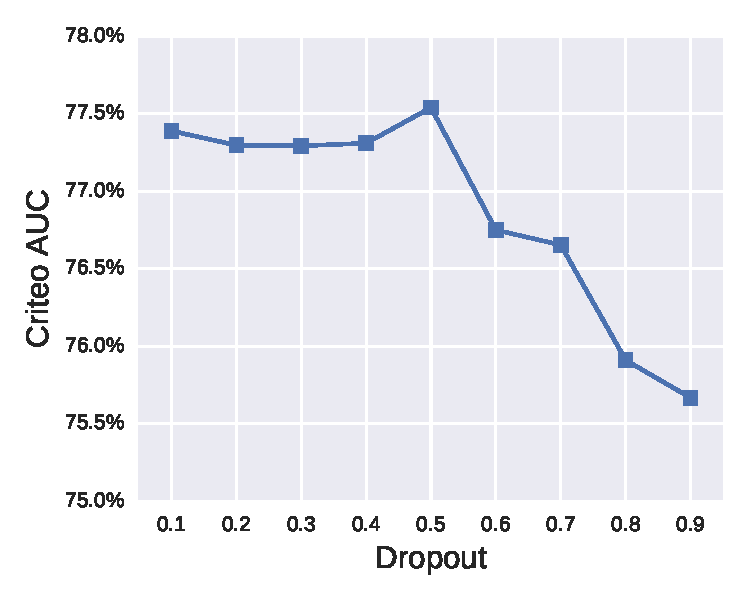
\includegraphics[width=0.7\columnwidth]{figure/drop-auc-2.pdf}
\vspace{-5pt}	
\caption{AUC Comparison of Dropout (OPNN).}\label{fig:drop-auc}
\vspace{-5pt}	
\end{figure}

%The reason why we choose 10-order factorization in FM and 10-order embedding layers in neural network models is simple: all of these models have linear complexity with respect to the order and, besides, this table compares shallow neural networks only (FNN: 4 layers, CCPM: 4 layers, PNNs: 5 layers), the factor of network depth that is deeper than 5 will be discussed in Section~\ref{sec:arch}.

Firstly, we focus on the AUC performance. The overall results in Table \ref{tab:perf-criteo} and \ref{tab:perf-ipinyou} illustrate that (i) FM outperforms LR, demonstrating the effectiveness of feature interactions; (ii) Neural networks outperform LR and FM, which validates the importance of high-order latent patterns; (iii) PNNs perform the best on both Criteo and iPinYou datasets. As for log loss, RMSE and RIG, the results are similar.




We also conduct t-test between our proposed PNNs and the other compared models. Table~\ref{tab:pvalue} shows the calculated p-values under log loss metric on both datasets. The results verify that our models significantly improve the performance of user response prediction against the baseline models.

%Inspired by the better performance of FM than LR, we come up with the idea of product layers. Comparing PNNs with other neural networks, we find product layers expand neural network's capacity via quadratic feature combinations.

%We also find that: PNN-I and PNN-II have similar performance on the Criteo dataset. However, PNN-II outperforms PNN-I on the iPinYou dataset. We consider two main reasons here:

%1). Data is seriously imcomplete in the iPinYou dataset, which will be treated as zero input. In PNN-I, zero input results in zero output in the inner product layer, while in PNN-II, the superposition of all features discards zero input. Our experiments give the reason Figure~\ref{fig:train}: on the iPinYou dataset, PNN-II increases steadily, while PNN-I increases with fluctuations.

%2). The iPinYou dataset is seriously incomplete, e.g. some data instances may have 60 feature values, while some others only have 20. For the consistance of input, we have to feed null values sometimes. The introduced null values make no effects on the outer product layer for superposition operation, however, result in zero outputs in the inner product layer. On one hand, these zero terms might increase complexity, but may conflict with matrix factorization assumptions on the other hand, making PNN-II more robust than PNN-I.

We also find that PNN*, which is the combination of IPNN and OPNN, has no obvious advantages over IPNN and OPNN on AUC performance.
We consider that IPNN and OPNN are sufficient to capture the feature interactions in multi-field categorical data.
%We consider the reason is that PNN* has higher complexity, thus suffers from overfitting more seriously.
%\kan{I think the meaning has conflicts.}

%Even though CCPM does not have extraordinary performance, it converges fast. The reason is simple, one convolutional layer in CCPM shares one single kernel, and flexible pooling layers selects better combinations \cite{liu2015convolutional}. In consequence, CCPM has fewer parameters, making it efficient and steady in training.

%However, there are two factors that restrict CCPM's performance: 1) Convolutional operation highly relies on the input sequence, in other words, exchanging features may yield completely different models. Besides, it is impossible to try every permutation manually. 2) Sharing kernels among features still need validation. As is a common sense in image processing, sharing kernels is based on spatial locality and invariance. While the ad data we use do not have this property.

%We find that all the neural networks converge more quickly than LR and FM. We also observe that our two proposed PNNs have better convergence than other network models. And OPNN empirically performs the best.

\begin{figure}[t]
	\centering
	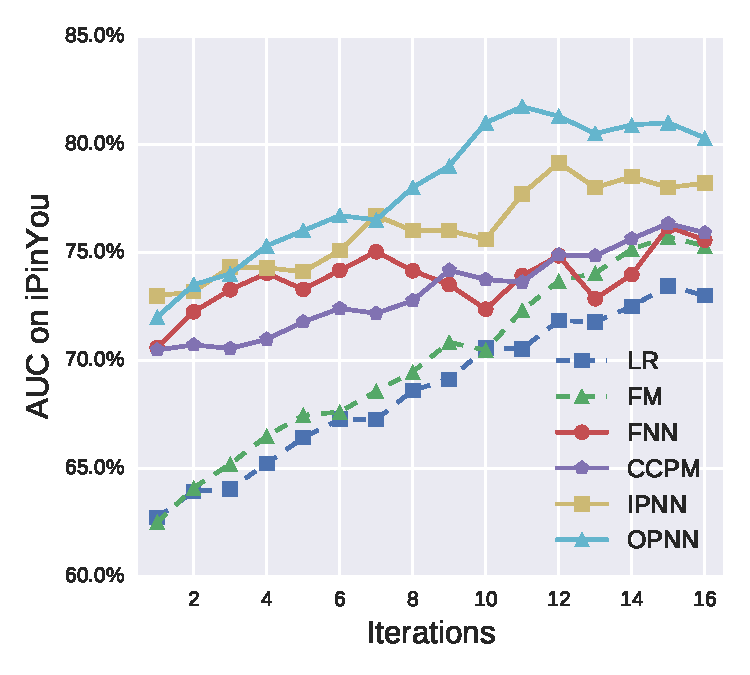
\includegraphics[width=0.7\columnwidth]{figure/train-2.pdf}
	\caption{Learning Curves on the iPinYou Dataset.}\label{fig:train}
\end{figure}

Figure \ref{fig:train} shows the AUC performance with respect to the training iterations on iPinYou dataset. We find that network models converge more quickly than LR and FM. We also observe that our two proposed PNNs have better convergence than other network models.
%And OPNN empirically performs the best.

\subsection{Ablation Study on Network Architecture}\label{sec:arch}
In this section, we discuss the impact of neural network architecture.
For IPNN and OPNN,
%there are 4 factors, sufficiently determining the neural networks' architecture:
we take three hyper-parameters (or settings) into consideration:
(i) embedding layer size, (ii) network depth and (iii) activation function. Since CCPM shares few similarities with other neural networks and PNN* is just a combination of IPNN and OPNN, we only compare FNN, IPNN and OPNN in this section.

\subsubsection{Embedding Layer}
%In this section, we study the embedding layer.
%Neural networks are widely used to learn distributed node representations.
The embedding layer is to convert sparse binary inputs to dense real-value vectors.
Take word embedding as an example \cite{mikolov2013distributed},
%distinct words are transformed into low-dimensional real-valued feature vectors via shallow networks.
an embedding vector contains the information of the word and its context, and indicates the relationships between words.
%Different from natural language, an IR data instance has multiple fields of categorical data.

We take the idea of embedding layer from \cite{zhang2016deep}. In this paper, the latent vectors learned by FM are explained as node representations, and the authors use a pre-trained FM to initialize the embedding layers in FNN. Thus the factorization order of FM keeps consistent with the embedding order.
%We implement the embedding layers according to this idea.
%, we implement field-wise embedding layers fully connected within each field.
%For this reason, we employ an embedding layer field-wisely connected to the multi-field categorical input. More specifically, the embedding layer can be divided into several parts, each input field fully connected with one part.

The input units are fully connected with the embedding layer within each field.
%Here we give an example to show the difference. Suppose that a data instance has $N$ fields as input, the input is fully connected with the embedding layer within each field. Field $n$ has dimension $D$ and $D$ input units are fully connected with $M$ embedding nodes. These links form a $D \times M$ matrix $m$. Multiplied with $m$, field $n$ is converted to a real valued vector with order $M$. Because the input is one-hot encoded, field $n$ has only one positive unit, thus multiplying $n$ with $m$ is equivalent to slicing a row vector in $m$. In consequence, $N$ row vectors are picked out representing $N$ input fields.
%Because the complexity of the embedding layer is linear with respect to the embedding order,
%Besides, the embedding order in network is the same with the factorization order in FM.
We compare different orders, like 2, 10, 50 and 100. However, when the order grows larger, it is harder to fit the parameters in memory, and the models are much easier to over-fit.
In our experiments, we take 10-order embedding in neural networks.

%We also explore the impacts of network initialization. Our network layers are all initialized randomly close to 0. We compare our models with or without pre-training of the embedding layer \cite{zhang2016deep}, and the result shows slight difference.

\subsubsection{Network Depth}%\label{sec:net-depth}

\begin{figure}[t]
	\centering
	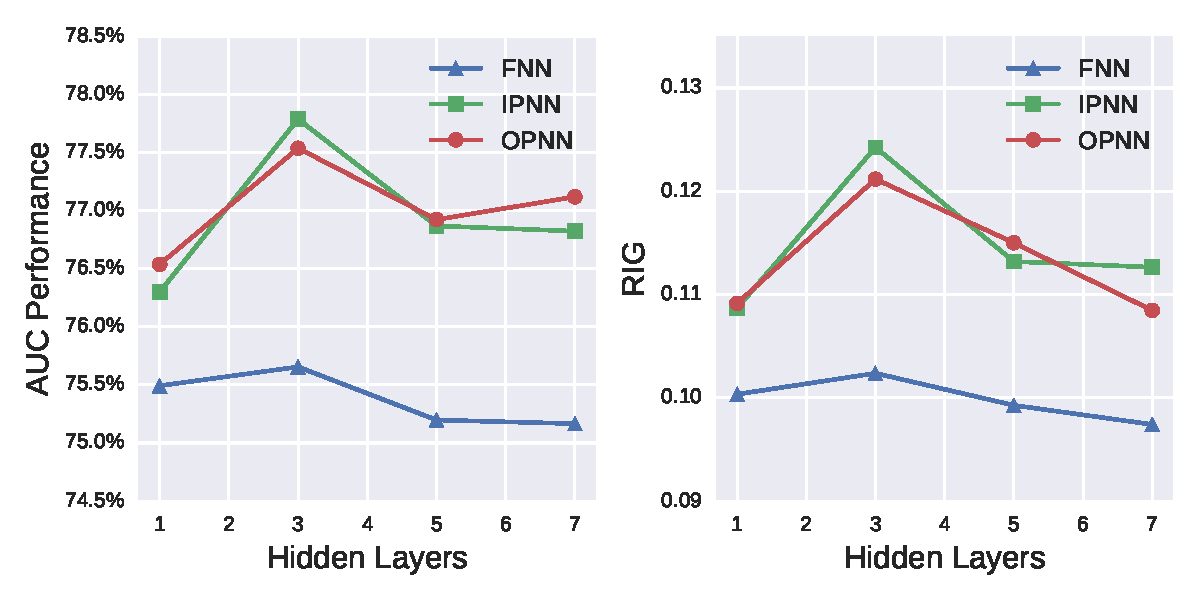
\includegraphics[width=0.5\textwidth]{figure/nn-depth-short-2.pdf}
	\caption{Performance Comparison over Network Depths.}\label{fig:depth}
\end{figure}

We also explore the impact of network depth by adjusting the number of hidden layers in FNN and PNNs.
%In FNN or PNN, the network consists of one embedding layer and several fully connected layers. PNN employs one more product layer. With \{1, 3, 5, 7\} hidden layers, the depth of FNN becomes \{2, 4, 6, 8\}, and the depth of PNN becomes \{3, 5, 7, 9\} correspondingly.
We compare different number of hidden layers: 1, 3, 5 and 7. Figure \ref{fig:depth} shows the performance as network depth grows. Generally speaking, the networks with 3 hidden layers have better generalization on the test set.
%This result depends on the data scale and data distribution as well as the dropout regularization.
%In contrast, adding convolution layers in CCPM increases its performance \cite{liu2015convolutional}. %\kan{needs revision}

For convenience, we call convolution layers and product layers as representation layers.
%and we call fully connected layers as forwarding layers.
%We find representation layers play a crucial role in learning data representations.
%while forwarding layers are able to explore more complicated combinations.
%And of course, the performance of feed-forward layers heavily relies on the data representations learned by the representation layers.
% Network structure should represent data characteristics. Besides, a deeper model is easier to overfit and harder to train.
%We find that the studied ad data have complex feature interactions, with relatively shallow hierarchy.
%In this experiment, for each of FNN and PNN models with restricted data representation, too many forwarding layers increase training complexity.
These layers can capture complex feature patterns using fewer parameters, thus are efficient in training, and generalize better on the test set.

%Finally, we conclude that deep neural network relies its advantages on efficient learning of data representations.

\subsubsection{Activation Function}
We compare three mainstream activation functions: $\sigmoid(x) = \frac{1}{1+e^{-x}}$, $\tanh(x) = \frac{1 - e^{-2x}}{1 + e^{-2x}}$, and $\relu(x) = \max(0, x)$.
%Sigmoid and tanh are in the sigmoidal family, while relu has quite different characteristics.
Compared with the sigmoidal family, relu function has the advantages of sparsity and efficient gradient, which is possible to gain more benefits on multi-field categorical data.
%\begin{equation}
%\begin{split}
%\sigma(x) & = \frac{1}{1+e^{-x}} \\
%\tanh(x) & = \frac{1 - e^{-2x}}{1 + e^{-2x}} \\
%\relu(x) & = \max(0, x)
%\end{split}
%\end{equation}

\begin{figure}[t]
	\centering
	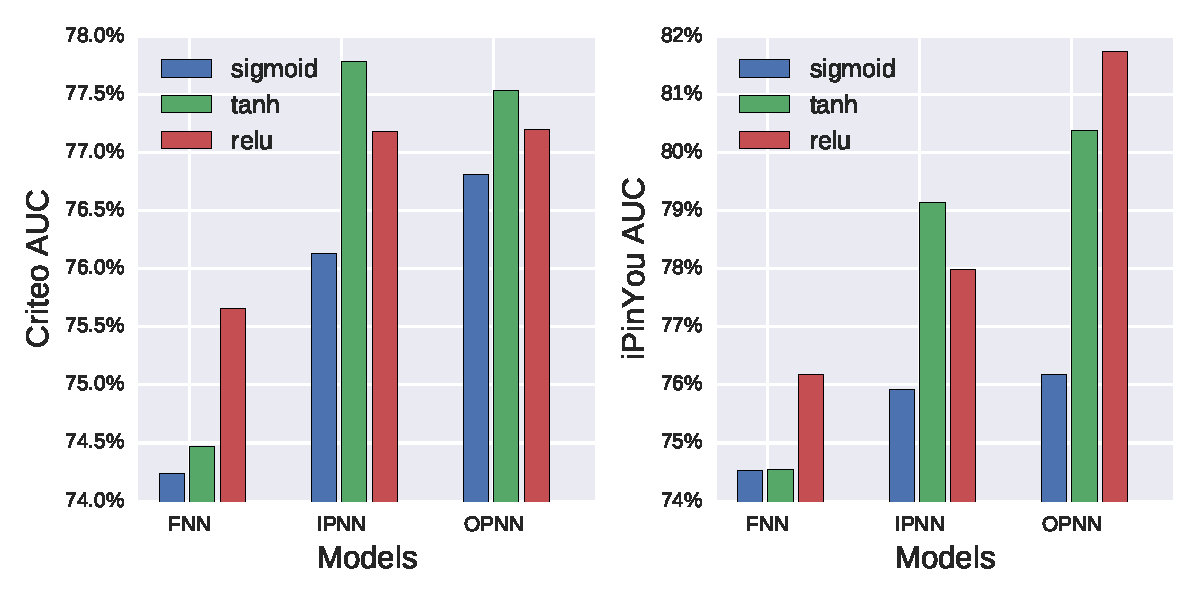
\includegraphics[width=0.5\textwidth]{figure/nn-auc-2.pdf}
	\caption{AUC Comparison over Various Activation Functions.}\label{fig:act}
\end{figure}

Figure \ref{fig:act} compares these activation functions on FNN, IPNN and OPNN. From this figure, we find that tanh has better performance than sigmoid. This is supported by \cite{zhang2016deep}.
%. Besides, different from relu's sparse activation,
%\cite{zhang2016deep} proves tanh's advantages on multi-field categorical data. We also find the relu function with considerable performance.
Besides tanh, we find relu function also has good performance. Possible reasons include: (i) Sparse activation, nodes with negative outputs will not be activated; (ii) Efficient gradient propagation, no vanishing gradient problem or exploding effect; (iii) Efficient computation, only comparison, addition and multiplication.

\section{Conclusion and Future Work}\label{sec:conclusion}
In this paper, we proposed a deep neural network model with novel architecture, namely Product-based Neural Network, to improve the prediction performance of DNN working on categorical data. And we chose CTR estimation as our working example. By exploration of feature interactions, PNN
%can not only learn promising data representation on sparse features, but also capture the latent interactive patterns.
is promising to learn high-order latent patterns on multi-field categorical data.
We designed two types of PNN: IPNN based on inner product and OPNN based on outer product. We also discussed solutions to reduce complexity, making PNN efficient and scalable. Our experimental results demonstrated that PNN outperformed the other state-of-the-art models in 4 metrics on 2 datasets. To sum up, we obtain the following conclusions: (i)
%Compared with LR and FM, PNN can learn more complicated patterns.
By investigating feature interactions, PNN gains better capacity on multi-field categorical data. (ii) Being both efficient and effective, PNN outperforms major state-of-the-art models. (iii)
%As for network architecture: data representation contributes more than network depth, and network structure should also depend on data characteristics.\rocky{these three points are experiment result or paper conclusion?}
%Instead of learning feature representations, PNN attempts to learn the rules, which may be more important on categorical data.
Analogous to ``AND''/``OR'' gates, the product/add operations in PNN
provide a potential strategy for data representation, more specifically, rule representation.

In the future work, we will explore PNN with more general and complicated product layers. Besides, we are interested in explaining and visualizing the feature vectors learned by our models. We will investigate their properties, and further apply these node representations to other tasks.
%As discussed in section \ref{sec:general-pnn}, inner/outer product are just two implementations of vector product.
%investigate various kernel methods to explore different data representations and interactions. We will also explore more properties of the embedding layers, to better model the characteristics of both the numerical and the sparse multi-field categorical features.

%Product layers take vector inputs with same order, requiring extra efforts in feature processing. Thus the next step, we want to generalize our PNN models. Data determines strcture, thus we need further study Ad. data characteristics. Moreover, dispite the disadvantages illustrated in Section~\ref{perf}, we find CCPM efficient in learning complicated patterns from sparse data. Thus we would like to improve CCPM by discarding sequence reliance.

% use section* for acknowledgment
%\section*{Acknowledgment}
%We would like to thank Prof. Yu's great help on this work, without his generous instructions and experimental support, this work can never be done properly. It's Prof. Yu's rigorous scientific attitude pushes us to improve our experiments. And we appreciate Weinan Zhang's work and proposal. Besides, his benchmark on the iPinYou dataset saves us a lot of time in experiments. We also thank Kan Ren's help in experimental design and model implementation. We thank for Han Cai's and Yun Cao's great help in formula derivation. Thanks to their generous help, we are able to reduce our models' complexity. We thank for other APEX Lab members' contributions in discussion and valuable advices.

\bibliographystyle{IEEEtran}
\bibliography{main}

% that's all folks
\end{document}
